\begin{blocksection}
\question Here, a \textbf{heuristic} is an educated guess of the distance from the node to the goal. For example, for node $S$, we see that $h=6$.  This means that it is estimated that $S$ is 6 units away from $G$. 

Find the path from the start, $S$, to the goal, $G$, when running
each of the following algorithms.

\begin{center}
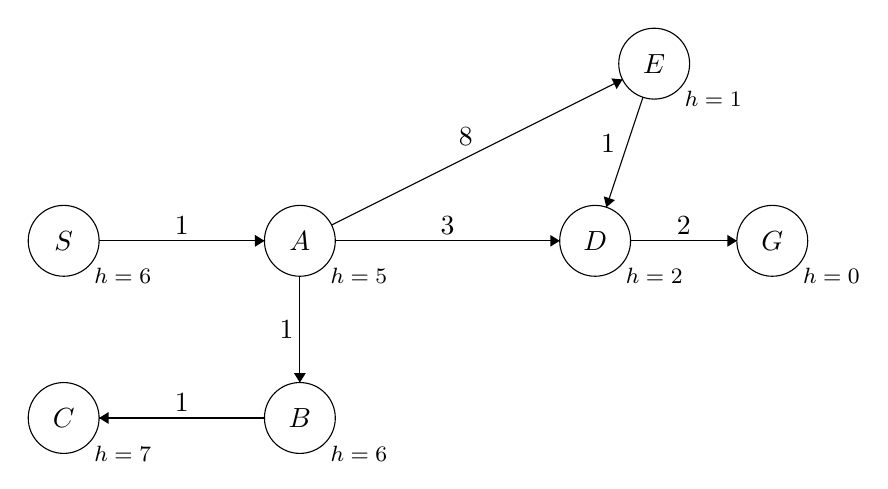
\begin{tikzpicture}[scale=0.15]
\tikzstyle{every node}+=[inner sep=0pt]
\draw (60,-15) circle (3);
\draw (60,-15) node {$E$};
\draw (65,-18) node {\footnotesize $h = 1$};
\draw (10,-30) circle (3);
\draw (10,-30) node {$S$};
\draw (15,-33) node {\footnotesize $h = 6$};
\draw (30,-30) circle (3);
\draw (30,-30) node {$A$};
\draw (35,-33) node {\footnotesize $h = 5$};
\draw (30,-45) circle (3);
\draw (30,-45) node {$B$};
\draw (35,-48) node {\footnotesize $h = 6$};
\draw (55,-30) circle (3);
\draw (55,-30) node {$D$};
\draw (60,-33) node {\footnotesize $h = 2$};
\draw (70,-30) circle (3);
\draw (70,-30) node {$G$};
\draw (75,-33) node {\footnotesize $h = 0$};
\draw (10,-45) circle (3);
\draw (10,-45) node {$C$};
\draw (15,-48) node {\footnotesize $h = 7$};
\draw (13,-30) -- (27,-30);
\fill (27,-30) -- (26.2,-29.5) -- (26.2,-30.5);
\draw (20,-29.5) node [above] {$1$};
\draw (30,-33) -- (30,-42);
\fill (30,-42) -- (30.5,-41.2) -- (29.5,-41.2);
\draw (29.5,-37.5) node [left] {$1$};
\draw (27,-45) -- (13,-45);
\fill (13,-45) -- (13.8,-45.5) -- (13.8,-44.5);
\draw (20,-44.5) node [above] {$1$};
\draw (33,-30) -- (52,-30);
\fill (52,-30) -- (51.2,-29.5) -- (51.2,-30.5);
\draw (42.5,-29.5) node [above] {$3$};
\draw (32.68,-28.66) -- (57.32,-16.34);
\fill (57.32,-16.34) -- (56.38,-16.25) -- (56.82,-17.15);
\draw (44.04,-22) node [above] {$8$};
\draw (59.05,-17.85) -- (55.95,-27.15);
\fill (55.95,-27.15) -- (56.68,-26.55) -- (55.73,-26.24);
\draw (56.73,-21.8) node [left] {$1$};
\draw (58,-30) -- (67,-30);
\fill (67,-30) -- (66.2,-29.5) -- (66.2,-30.5);
\draw (62.5,-29.5) node [above] {$2$};
\end{tikzpicture}
\end{center}

\begin{solution}
Note that uniform cost search and greedy search are not a part of the course.
The algorithms for all 3 of these searches are extremely similar, the only
difference being the priority given to a key and whether or not we need the
cumulative distance to a vertex.
\end{solution}

\begin{parts}
\part Uniform cost search is the same as Dijkstra's, except that you stop the procedure once you reach your goal state.  
Which path does uniform cost search return?
\begin{solution}[1in]
$S - A - D - G$

From the starting node, choose the path that has the least cost, go to that
node, and repeat until we reach the goal node. We choose the lowest
\emph{backward cost}.

Note that this is very similar to Dijkstra's, just a little more general. We
keep a priority-queue fringe that keeps track of paths. At each step, we remove
the shortest path from the fringe and add its children to the fringe, trying
all paths in increasing cost order until we reach G.
\end{solution}

\part In greedy search, we ignore edge weights and only consider the heuristics to decide which node to go to next.  Just a note, we don't add heuristics together because they are an estimate of the distance to the goal.
Which path does greedy search return?
\begin{solution}[1in]
$S - A - E - D - G$ 

From the starting node, travel to the next node with the lowest value returned
by the heuristic function until we reach the goal node. We choose the path with
the lowest \emph{forward cost}.
\end{solution}

\part A* is an algorithm that uses both heuristics and edge weights to find the shortest path to a goal.  For A* to work, heuristics must be an underestimate of the true distance to the goal.  
Which path does A* search return?
\begin{solution}[1in]
$S - A - D - G$

At each node, we choose the next node that has the lowest sum of the path cost
and $h(\cdot)$ value. This is essentially uniform cost search and greedy search
combined.

\end{solution}
\end{parts}
\end{blocksection}
